\chapter{INTRODUÇÃO}

Para o contexto de desenvolvimento de software, segurança da informação é a área que potencialmente define entre o sucesso ou fracasso de uma aplicação. E no caso de inúmeras aplicações web com elevado tráfego, ela aparece apenas em uma reflexão tardia. Atualmente navegadores web como \textit{Chrome}, \textit{Firefox} e \textit{Safari} ativamente notificam o usuário de falhas chave nesse quesito como certificação HTTPS, tornando ações fundamentais como transações (quando inseguras) na web uma área de atenção redobrada para consumidores finais. O valor de medidas que remediam falhas nessa área também faz com que poucos sites discorram sobre seus segredos de segurança, informações consideradas de altíssimo valor. Isso torna complicado assegurar como é o estado atual de vulnerabilidades web hoje em dia. Nesse sentido busca-se, com esse trabalho, elucidar um pouco o estado atual das medidas publicadas para conter o avanço de ataques à tais aplicações, e introduzir uma contribuição para esse panorama na forma de uma nova ferramenta \textit{open-source}.

Historicamente, o conceito de vulnerabilidade na Internet modificou-se consideravelmente. A \textit{World Wide Web} consistia, nos seus primórdios, de web sites cujas funções principais eram essencialmente fornecer ao usuário final documentos estáticos de informação, inicialmente definida nos anos 1960 como um meio de pesquisadores do governo compartilharem informação. O fluxo de informação era de via única, no qual o conteúdo saía do servidor ao usuário final, apenas. Autenticação não era uma realidade para a maioria dos sites, pois não havia necessidade. Cada usuário que visitasse uma página web recebia a mesma informação. \cite{stuttard_web_nodate} Vulnerabilidades nessa época consistiam principalmente em numerosos \textit{exploits} sob software de servidores, para distribuir \textit{warez} (software ilegalmente copiado e distribuído) ou meramente deturpar a parte visual de um site (prática conhecida como \textit{defacing}).

Em contraste a isso, na atualidade a maioria dos sites na Internet consistem de aplicações robustas com diversas funcionalidades que eram inconcebíveis na época, dependendo de um fluxo de informação de via dupla entre cliente e servidor. Usuários precisam, incontáveis vezes, de credenciais para realizar cadastros que cuidam das mais modestas trocas de informações como postagens em fóruns de discussão até os mais sensíveis dados bancários transacionais. Surge a necessidade concreta de gerenciadores de senha de ponta, muitas vezes oferecidos pelo próprio navegador web (embora inseguro). Além disso, torna-se onipresente a linguagem de script/programação \textit{JavaScript} moderna, que fornece a essas aplicações um dinamismo inerente, tanto na parte visual do cliente (\textit{front-end}), como na parte funcional do servidor (\textit{back-end}, através de tecnologias como Node.js). Cada internauta torna-se diferente do próximo, transformando-se a interatividade de sites, aumentando o fluxo de dados que dependem do usuário e conteúdo como imagens e vídeos na internet.

Esses novos meios trazem novas possibilidades de ataque de agentes maliciosos, trazendo consigo uma gama de técnicas novas a serem utilizadas. Não obstante, surgem também técnicas de defesa avançadas que muitas vezes podem remediar casos graves de vulnerabilidade. Um tipo de componente amplamente usado para tratar vulnerabilidades em uma dada aplicação web é um \textit{Web Application Firewall} - responsável por monitorar tráfego de internet que é conduzido pela aplicação, permitindo ou bloqueando pacotes que possam ser potencialmente maliciosos. E recentemente, com o advento de técnicas de Aprendizado de Máquina, uma série de \textit{Web Application Firewalls} baseados nesse subcampo de Inteligência Artificial foram criados com o intuito não apenas de explorar a área em si, como também de gerar \textit{Firewalls} mais robustos e capazes de deter tráfego de ataques web. 

Buscando-se como alvo de pesquisa as mais aplicáveis defesas, propõe-se como uma nova solução nesse subcampo o software extensível e \textit{open-source}  \textbf{wafamole++}, baseado no \textbf{WAF-A-MoLE} \cite{valenza_waf--mole_2020} inicialmente demonstrado por autores da Universidade de Genebra, uma ferramenta de segurança que permite a testagem desses \textit{firewalls} de ponta através de técnicas de \textit{fuzzing}, e um subsequente caminho para torná-los ainda mais robusto. 

Essa nova implementação surge das possibilidades de melhorias no \textit{WAF-A-MoLE} verificadas pelos autores - uma arquitetura engessada que dificultava o uso e reprodução da ferramenta, uma série de modelos de ataque faltantes que poderiam ser utilizados porém não foram, e uma lista de operadores de mutação (um aspecto chave do seu funcionamento, explicado mais adiante) que poderia ser ainda mais estendida. Para corrigir a mesma, foram criadas várias ferramentas auxiliares que possibilitam a um contribuidor ou usuário treinar (e testar) um \textit{Web Application Firewall} baseado em aprendizado de máquina mais facilmente, um \textit{wrapper} para qualquer classificador da biblioteca \verb+scikit-learn+ fora introduzido, e a eficiência do programa foi incrementada com novos operadores de mutação.

Nesse contexto, são então apresentados: 
\begin{alineas}
\item Revisão de literatura conduzida com o auxílio de ferramentas externas;
\item Um panorama dos resultados da pesquisa realizada;
\item Embasamento teórico para a compreensão plena de tecnologias empregadas;
\item Descrição da implementação, e técnicas de uma solução proposta pelos autores, intitulada de \textbf{wafamole++};
\item Testes realizados para a mesma e conclusões do processo como um todo.
\end{alineas}

% \begin{figure}[ht]
%     \centering
%     \caption{Evolução da adoção de JavaScript em aplicações web}
%     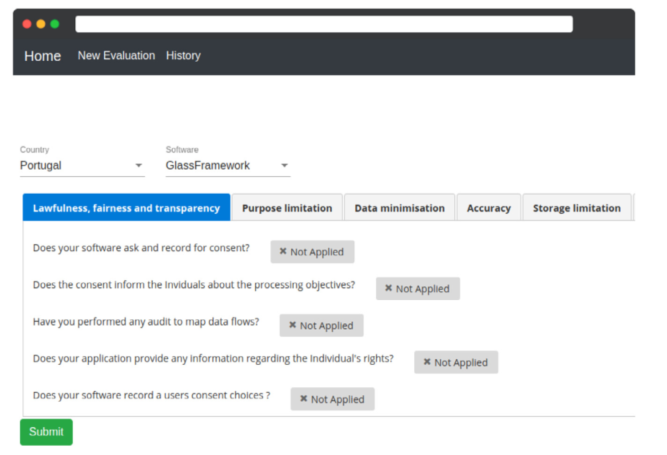
\includegraphics[width=14cm]{figuras/padres.png} 
%     \legend{Fonte: \href{https://www.sciencedirect.com/science/article/pii/S2352711021001515}{Fábio Pereira, Paul Crocker, Valderi R.Q. Leithardt et al via Scopus} (2022, p. TO-DO)}
%     \label{fig:internet} 
% \end{figure}

\bigskip
